\documentclass[tikz,border=2mm]{standalone}
\usepackage[T1]{fontenc}
\usepackage[swedish,english]{babel}
\usepackage{tikz}
\usetikzlibrary{arrows,positioning}
\usepackage{pgfplots}
\usepackage{amsmath,mathtools}
\usepgfplotslibrary{fillbetween}
\begin{document}
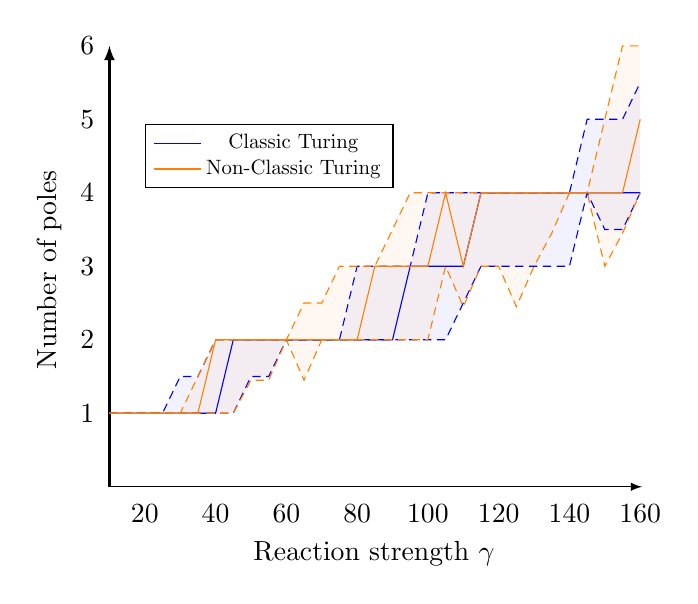
\begin{tikzpicture}
\begin{axis}[
    %hide axis,
    %axis lines* = left,
    %axis lines=left, xtick=\empty, ytick=\empty.
    axis line style={draw=none},
    tick style={draw=none},
    xticklabel style={yshift=-0.1mm},
    xmin = 8.5,
   xmax = 161,
    ymin = -0.1,
    ymax = 6,
    %grid=both,
    %xtick = {1,0.95,...,0.6},
    ytick = {1,...,6},    
    %xticklabels = {{zero},$\alpha$,$\varphi$},
   %xlabel style={at={(axis cs:0.61,7)},anchor=east,align=center},
    %ylabel style={at={(axis cs:1.00,35)},anchor=north,rotate=0},
	xlabel = {Reaction strength $\gamma$},
        ylabel = {Number of poles},
    legend style={at={(axis cs:20,4.5)},anchor=west,cells={align=center},nodes={scale=0.75}},
    %x dir=reverse
    %legend entries = {Decreasing the inactivation rate $k_{-2}$}
]
%-------------------------------------------------------------------------------------------------
% AXES
\draw[->,-latex, thick] (axis cs: 10,0) -- (axis cs: 10,6); % y-axis
\draw[->,-latex] (axis cs: 10,0) -- (axis cs: 160.5,0); % x-axis
%-------------------------------------------------------------------------------------------------
%-------------------------------------------------------------------------------------------------
% Classical 
%-------------------------------------------------------------------------------------------------
\addplot[forget plot,densely dashed,color=blue,name path=UpnuOfPolesClassical] coordinates {
		(10.0000	,	1.0000	)
		(15.0000	,	1.0000	)
		(20.0000	,	1.0000	)
		(25.0000	,	1.0000	)
		(30.0000	,	1.5000	)
		(35.0000	,	1.5000	)
		(40.0000	,	2.0000	)
		(45.0000	,	2.0000	)
		(50.0000	,	2.0000	)
		(55.0000	,	2.0000	)
		(60.0000	,	2.0000	)
		(65.0000	,	2.0000	)
		(70.0000	,	2.0000	)
		(75.0000	,	2.0000	)
		(80.0000	,	3.0000	)
		(85.0000	,	3.0000	)
		(90.0000	,	3.0000	)
		(95.0000	,	3.0000	)
		(100.0000	,	4.0000	)
		(105.0000	,	4.0000	)
		(110.0000	,	4.0000	)
		(115.0000	,	4.0000	)
		(120.0000	,	4.0000	)
		(125.0000	,	4.0000	)
		(130.0000	,	4.0000	)
		(135.0000	,	4.0000	)
		(140.0000	,	4.0000	)
		(145.0000	,	5.0000	)
		(150.0000	,	5.0000	)
		(155.0000	,	5.0000	)
		(160.0000	,	5.5000	)
};

\addplot[color=blue] coordinates {
		(10.0000	,	1.0000	)
		(15.0000	,	1.0000	)
		(20.0000	,	1.0000	)
		(25.0000	,	1.0000	)
		(30.0000	,	1.0000	)
		(35.0000	,	1.0000	)
		(40.0000	,	1.0000	)
		(45.0000	,	2.0000	)
		(50.0000	,	2.0000	)
		(55.0000	,	2.0000	)
		(60.0000	,	2.0000	)
		(65.0000	,	2.0000	)
		(70.0000	,	2.0000	)
		(75.0000	,	2.0000	)
		(80.0000	,	2.0000	)
		(85.0000	,	2.0000	)
		(90.0000	,	2.0000	)
		(95.0000	,	3.0000	)
		(100.0000	,	3.0000	)
		(105.0000	,	3.0000	)
		(110.0000	,	3.0000	)
		(115.0000	,	4.0000	)
		(120.0000	,	4.0000	)
		(125.0000	,	4.0000	)
		(130.0000	,	4.0000	)
		(135.0000	,	4.0000	)
		(140.0000	,	4.0000	)
		(145.0000	,	4.0000	)
		(150.0000	,	4.0000	)
		(155.0000	,	4.0000	)
		(160.0000	,	4.0000	)
};

\addplot[forget plot,densely dashed,color=blue,name path=DownnuOfPolesClassical] coordinates {
		(10.0000	,	1.0000	)
		(15.0000	,	1.0000	)
		(20.0000	,	1.0000	)
		(25.0000	,	1.0000	)
		(30.0000	,	1.0000	)
		(35.0000	,	1.0000	)
		(40.0000	,	1.0000	)
		(45.0000	,	1.0000	)
		(50.0000	,	1.5000	)
		(55.0000	,	1.5000	)
		(60.0000	,	2.0000	)
		(65.0000	,	2.0000	)
		(70.0000	,	2.0000	)
		(75.0000	,	2.0000	)
		(80.0000	,	2.0000	)
		(85.0000	,	2.0000	)
		(90.0000	,	2.0000	)
		(95.0000	,	2.0000	)
		(100.0000	,	2.0000	)
		(105.0000	,	2.0000	)
		(110.0000	,	2.5000	)
		(115.0000	,	3.0000	)
		(120.0000	,	3.0000	)
		(125.0000	,	3.0000	)
		(130.0000	,	3.0000	)
		(135.0000	,	3.0000	)
		(140.0000	,	3.0000	)
		(145.0000	,	4.0000	)
		(150.0000	,	3.5000	)
		(155.0000	,	3.5000	)
		(160.0000	,	4.0000	)
};
\addplot[blue!50,opacity=0.1,forget plot] fill between[of=UpnuOfPolesClassical and DownnuOfPolesClassical];

\addlegendentry{Classic Turing}% Add to legend
%-------------------------------------------------------------------------------------------------
% Non-classical
%-------------------------------------------------------------------------------------------------
\addplot[forget plot,densely dashed,color=orange,name path=UpnuOfPolesNonClassical] coordinates {
		(10.0000	,	1.0000	)
		(15.0000	,	1.0000	)
		(20.0000	,	1.0000	)
		(25.0000	,	1.0000	)
		(30.0000	,	1.0000	)
		(35.0000	,	1.5000	)
		(40.0000	,	2.0000	)
		(45.0000	,	2.0000	)
		(50.0000	,	2.0000	)
		(55.0000	,	2.0000	)
		(60.0000	,	2.0000	)
		(65.0000	,	2.5000	)
		(70.0000	,	2.5000	)
		(75.0000	,	3.0000	)
		(80.0000	,	3.0000	)
		(85.0000	,	3.0000	)
		(90.0000	,	3.5000	)
		(95.0000	,	4.0000	)
		(100.0000	,	4.0000	)
		(105.0000	,	4.0000	)
		(110.0000	,	4.0000	)
		(115.0000	,	4.0000	)
		(120.0000	,	4.0000	)
		(125.0000	,	4.0000	)
		(130.0000	,	4.0000	)
		(135.0000	,	4.0000	)
		(140.0000	,	4.0000	)
		(145.0000	,	4.0000	)
		(150.0000	,	5.0000	)
		(155.0000	,	6.0000	)
		(160.0000	,	6.0000	)
};

\addplot[color=orange] coordinates {
		(10.0000	,	1.0000	)
		(15.0000	,	1.0000	)
		(20.0000	,	1.0000	)
		(25.0000	,	1.0000	)
		(30.0000	,	1.0000	)
		(35.0000	,	1.0000	)
		(40.0000	,	2.0000	)
		(45.0000	,	2.0000	)
		(50.0000	,	2.0000	)
		(55.0000	,	2.0000	)
		(60.0000	,	2.0000	)
		(65.0000	,	2.0000	)
		(70.0000	,	2.0000	)
		(75.0000	,	2.0000	)
		(80.0000	,	2.0000	)
		(85.0000	,	3.0000	)
		(90.0000	,	3.0000	)
		(95.0000	,	3.0000	)
		(100.0000	,	3.0000	)
		(105.0000	,	4.0000	)
		(110.0000	,	3.0000	)
		(115.0000	,	4.0000	)
		(120.0000	,	4.0000	)
		(125.0000	,	4.0000	)
		(130.0000	,	4.0000	)
		(135.0000	,	4.0000	)
		(140.0000	,	4.0000	)
		(145.0000	,	4.0000	)
		(150.0000	,	4.0000	)
		(155.0000	,	4.0000	)
		(160.0000	,	5.0000	)
};

\addplot[forget plot,densely dashed,color=orange,name path=DownnuOfPolesNonClassical] coordinates {
		(10.0000	,	1.0000	)
		(15.0000	,	1.0000	)
		(20.0000	,	1.0000	)
		(25.0000	,	1.0000	)
		(30.0000	,	1.0000	)
		(35.0000	,	1.0000	)
		(40.0000	,	1.0000	)
		(45.0000	,	1.0000	)
		(50.0000	,	1.4500	)
		(55.0000	,	1.4500	)
		(60.0000	,	2.0000	)
		(65.0000	,	1.4500	)
		(70.0000	,	2.0000	)
		(75.0000	,	2.0000	)
		(80.0000	,	2.0000	)
		(85.0000	,	2.0000	)
		(90.0000	,	2.0000	)
		(95.0000	,	2.0000	)
		(100.0000	,	2.0000	)
		(105.0000	,	3.0000	)
		(110.0000	,	2.4500	)
		(115.0000	,	3.0000	)
		(120.0000	,	3.0000	)
		(125.0000	,	2.4500	)
		(130.0000	,	3.0000	)
		(135.0000	,	3.4500	)
		(140.0000	,	4.0000	)
		(145.0000	,	4.0000	)
		(150.0000	,	3.0000	)
		(155.0000	,	3.4500	)
		(160.0000	,	4.0000	)
};
\addplot[orange!50,opacity=0.1,forget plot] fill between[of=UpnuOfPolesNonClassical and DownnuOfPolesNonClassical];

\addlegendentry{Non-Classic Turing}% Add to legend
\end{axis}

\end{tikzpicture}



\end{document}
